\documentclass[12pt,letterpaper,oneside]{article}
\newcommand{\JASASubmission}{}
\usepackage[T1]{fontenc}
\usepackage[utf8]{inputenc}
\usepackage{lmodern,microtype}
\usepackage[margin=1in]{geometry}
\usepackage{amsmath,amssymb,amsthm,mathtools,mathrsfs}
\usepackage{graphicx,booktabs,array,enumitem}
\usepackage[round,authoryear]{natbib}
\usepackage{setspace}
\usepackage{xr-hyper}
\usepackage[colorlinks=true,linkcolor=blue,citecolor=blue,urlcolor=blue]{hyperref}
\usepackage{bookmark}
\allowdisplaybreaks
\setlength{\emergencystretch}{2em}
\setlist{topsep=3pt,itemsep=2pt}
\newtheorem{theorem}{Theorem}
\ifdefined\JASASubmission
\newtheorem{proposition}{Proposition}
\newtheorem{lemma}{Lemma}
\newtheorem{corollary}{Corollary}
\else
\newtheorem{proposition}[theorem]{Proposition}
\newtheorem{lemma}[theorem]{Lemma}
\newtheorem{corollary}[theorem]{Corollary}
\fi
\theoremstyle{remark}
\ifdefined\JASASubmission
\newtheorem{remark}{Remark}
\else
\newtheorem{remark}[theorem]{Remark}
\fi
\newcommand{\EE}{\mathbb E}
\newcommand{\PP}{\mathbb P}
\newcommand{\cR}{\mathfrak R}
\newcommand{\cS}{\mathscr S}
\newcommand{\cC}{\mathscr C}
\newcommand{\cN}{\mathcal N}
\newcommand{\ind}{\mathbf 1}
\newcommand{\logp}{\log_+}
\DeclareMathOperator{\kl}{kl}
\DeclareMathOperator{\TV}{TV}
\DeclareMathOperator*{\argmax}{arg\,max}
\DeclareMathOperator*{\argmin}{arg\,min}

% JASA submission formatting, based on the ASA Journals Production Office
% guide: https://files.taylorandfrancis.com/asa-style-guide.pdf
% Checked 2026-10-13. Journal-specific author instructions were inaccessible.
% The body spacing factor 1.8 was explicitly requested by the author.
% The title/abstract page uses single spacing and headings use normal
% title capitalization, following JASA-template/mab_aa_main.tex and the
% author's correction (2026-10-13).
% This file is used by the main manuscript only.
\geometry{letterpaper,margin=1in}
\usepackage{xurl}
\urlstyle{same}
\usepackage{titlesec}
\usepackage{caption}
\usepackage[section]{placeins}
\renewcommand{\topfraction}{0.95}
\renewcommand{\bottomfraction}{0.9}
\renewcommand{\textfraction}{0.05}
\renewcommand{\floatpagefraction}{0.6}
\setstretch{1.8}
\setlength{\parindent}{2em}
\setlength{\parskip}{0pt}
\pagestyle{plain}
\titleformat{\section}{\normalfont\large\bfseries\raggedright\hyphenpenalty=10000\exhyphenpenalty=10000}{\thesection.}{0.6em}{}
\titleformat{\subsection}{\normalfont\normalsize\bfseries}{\thesubsection}{0.6em}{}
\titleformat{\subsubsection}{\normalfont\normalsize\itshape}{\thesubsubsection}{0.6em}{}
\setcounter{secnumdepth}{2}
\setcitestyle{authoryear,round,semicolon,aysep={},yysep={,}}
\setlength{\bibhang}{2em}
\setlength{\bibsep}{0pt}
\renewcommand{\bibfont}{\normalsize}
\captionsetup{font={normalsize,stretch=1.8},labelfont=normalfont,
  labelsep=period,justification=raggedright,singlelinecheck=false}
\captionsetup[figure]{position=bottom}
\captionsetup[table]{position=top}
\hypersetup{hidelinks,
  pdftitle={The Temporal Geometry of Bandits With Arriving Arms},
  pdfauthor={},
  pdfkeywords={Adaptive allocation; dynamic regret; minimax risk; sequential experimentation; sleeping bandit}}
\makeatletter
\AtBeginDocument{\typeout{JASA-FORMAT font=\f@size pt; baseline=\the\baselineskip;
  paper=\the\paperwidth,\the\paperheight;
  text=\the\textwidth,\the\textheight}}
\renewcommand{\maketitle}{%
  \begin{center}
    {\setstretch{1}\LARGE\bfseries\@title\par}
  \end{center}
  \bigskip}
\renewenvironment{abstract}
  {\begin{center}\bfseries\abstractname\end{center}\quotation\normalsize}
  {\endquotation}
\makeatother

\title{The Temporal Geometry of Bandits With Arriving Arms}
\author{}
\date{}
\begin{document}
\begingroup
\setstretch{1}
\typeout{JASA-TITLE-PAGE baseline=\the\baselineskip; stretch=\baselinestretch}
\maketitle
\begin{abstract}
New actions can enter a sequential experiment after substantial evidence has accumulated for existing actions. Even with stationary reward distributions, the best available action can change. We characterize the minimax regret for each deterministic arrival schedule, allowing arbitrary finite batches. The rate is a sum of learning costs over the remaining-lifetime scales, and one causal MOSS policy attains it without knowing the endpoint or future arrivals while retaining every observation. An equivalent concave allocation problem makes schedule difficulty computable. A lifetime fixed point captures the Euclidean norm of the scale costs, whereas regret depends on their sum. Under independent random arrivals, the reward environment must remain fixed across schedules, and averaging the deterministic complexities can overstate minimax risk by a logarithmic factor. For fixed batch templates with a common random time stretch, we obtain a positive characterization by a computable truncated-lifetime functional; this result assumes a known endpoint and a stretch revealed by the first arrival. Numerical studies use compatible multiscale priors, an exact small-sample Bayes benchmark, separate clock and capacity interventions, and independent evaluation of common-gap mixtures. They identify both benefits and finite-sample costs of the algorithm's design choices.
\end{abstract}
\noindent\textit{Key Words:} Adaptive allocation; dynamic regret; minimax risk; sequential experimentation; sleeping bandit.
\vfill
\clearpage
\endgroup

\section{Introduction}
\subsection{Overview}
An experiment may continue while new actions become available. A product comparison can admit new designs; an allocation system can receive new candidates from an external development process. Existing observations remain informative about old actions, but each arrival introduces an alternative for which the system has no data. A natural objective is to limit the cumulative loss relative to the best action available at each decision time. We study this objective when actions remain available after entry and their reward distributions do not change.

The final number of actions gives an incomplete description of this problem. Consider an incumbent and $M$ new actions over $T$ rounds. If all new actions are present from the beginning, the usual worst-case learning cost is of order $\min\{T,\sqrt{MT}\}$. If the same actions arrive in the last round, the regret is at most one. With several arrival batches, neither the longest remaining lifetime nor the sum of the lifetimes generally determines the rate. Learning opportunities overlap, and several time scales can each contribute appreciably to the total loss. The question is therefore which feature of the entire arrival schedule measures its statistical difficulty.

We answer this question for every deterministic exogenous schedule. Each arm has an independent, stationary reward distribution supported on $[0,1]$. Arrivals can occur in arbitrarily large finite batches, and ties are allowed. We fix the schedule before maximizing expected regret over reward distributions. The benchmark chooses the available arm with largest mean at each round. In particular, the benchmark changes only because of arrivals, not because an existing reward distribution drifts.

The answer is a sum over remaining-lifetime scales. For a fixed endpoint, group the competing arms whose remaining lifetimes are between $2^{\ell-1}$ and $2^\ell$. A group containing $k_\ell$ arms contributes $\min\{2^\ell,\sqrt{k_\ell2^\ell}\}$. We show that the sum of these contributions equals the schedule-specific minimax regret up to universal multiplicative constants. A learner that knows neither the endpoint nor future arrivals achieves this rate. It uses a MOSS index with a clock that restarts when the number of competing arms doubles, while its sample counts and reward sums continue across every restart.

The main difficulty in the lower bound is to make the scale-specific testing problems coexist. Adding separate worst-case risks is invalid if their respective hard environments cannot occur together. Our construction selects a constant fraction of the relevant scale mass and places independent testing problems in disjoint time windows. The benchmark increments are summable, and the reference means do not reveal the outcomes of earlier tests. Information acquired before a testing window is included in its likelihood calculation. The upper bound faces a different issue: retaining observations prevents a conditional restart argument. We instead control all potential sample prefixes and charge each arm-count pair at most once.

A second expression makes the complexity computable without a dyadic grid. We maximize a clipped square-root objective over the fractional sample allocations allowed by the arrivals. The constraints are nested suffix capacities, and their optimizer has a lower-convex-hull representation. This is an instance of established nested resource allocation; its statistical role here is to identify a quantity equivalent to regret. The representation also gives exact stability properties, a sharp comparison with integer sample allocations and a precise explanation of diminishing marginal capacity when more arms are added.

The results distinguish several notions that are otherwise easy to conflate. A natural lifetime fixed point measures the Euclidean norm of the scale costs, while the minimax risk measures their sum. The two can differ by a factor of order $\sqrt{\log T}$. Retaining observations can reduce regret from squared-logarithmic to logarithmic order relative to an otherwise identical policy that erases them, even though both policies have the same minimax rate.

Random arrivals introduce another distinction. The reward environment must be fixed before the schedule is drawn, so separate least-favorable environments for different schedules cannot be combined. We first exhibit a law under which the average deterministic complexity grows logarithmically while joint minimax risk stays bounded. We then characterize the joint risk for fixed batch templates whose relative times share one random stretch. A truncated-lifetime functional identifies the amount of difficulty that a common environment can sustain across stretches. The endpoint is known in this result, and the first batch reveals the remaining schedule. The constants depend on the fixed template; the result does not address growing templates or arbitrary arrival laws.

The numerical studies follow these distinctions. Compatible product priors connect the multiscale lower construction to observed regret, with an exact Bayes calculation at small horizons. A factorial comparison separates clock changes from capacity calibration, while a matched pair isolates the effect of forgetting. Independent development and evaluation samples compare one reward environment across random schedules with environments chosen separately for each schedule. The studies include failures of the proposed index and retain the information differences between the policies being compared.

\subsection{Relation to Existing Work}
Stochastic sleeping bandits already allow changing availability sets. Ordering arms by their means makes the best-ordering comparator coincide with the best currently available arm. The AUER analysis of \citet{kleinberg2008sleeping} gives logarithmic bounds involving adjacent mean gaps for a finite pool and retains observations between appearances. Thus neither the comparator nor data retention is specific to the present model. \citet{gaillard2023sleeping} further relate sleeping internal regret to ordering regret under independent and identically distributed losses. Per-action guarantees such as those of \citet{nguyen2024sleeping} use another comparator: a fixed action on the rounds when it is active. These results do not by themselves give the constant-factor minimax risk for each specified monotone arrival schedule.

The growing-action setting is studied directly by \citet{ghalme2021ballooning}. Their ballooning-bandit formulation uses the best available arm and establishes both impossibility results and sublinear guarantees under assumptions on the arrival of a best arm, with further discussion of arrival rates. Their BL-MOSS procedure uses the horizon and arrival information to select a collection of arms and subsequently stops admitting new ones. Our characterization conditions on an arbitrary fixed schedule and maximizes over all bounded stationary reward laws. It imposes no tail assumption on the arrival of an optimal arm and requires no cutoff for admitting arms.

The index itself comes from MOSS \citep{audibert2009minimax}. Anytime minimax-optimal MOSS procedures for fixed arm sets were developed by \citet{degenne2016anytime}; the coexistence of minimax and instance-dependent guarantees also has substantial precedent, including \citet{menard2017minimax}. We use this literature as the local learning component. The contribution is the schedule-specific upper and lower characterization, with an upper-bound argument that permits clock recalibration while retaining observations as the arm pool grows. Our gap bound is not an instance-optimality result.

The allocation representation is related to separable convex optimization with nested constraints. \citet{vidal2016nested} explicitly derive lower-convex-hull solutions for shared-shape objectives, and \citet{vidal2019separable} treat nonsmooth convex objectives within a broader class. General submodularity results for concave optimization over polymatroids are available in \citet{he2012polymatroid}. We use these structures with explicit proofs for the present clipped square-root objective. The connection to bandit risk, rather than a new convex optimization algorithm, is the point of the representation.

\section{Arrival Geometry and Minimax Risk}\label{sec:geometry}
\subsection{Model and Information}
Arms have labels in a countable set. Fix a deterministic sequence of integer arrival times $\tau_i\ge1$, with
\[
 A_t=\{i:\tau_i\le t\},\qquad 1\le K_t:=|A_t|<\infty.
\]
At round $t$, the learner observes the entire new batch before choosing $I_t\in A_t$. Arm $i$ supplies a potential reward stream $(X_{i,n})_{n\ge1}$ of independent and identically distributed random variables with values in $[0,1]$ and mean $\mu_i$. Streams are independent across arms. The $n$th pull reveals $X_{i,n}$; all other rewards remain unobserved. Policy randomization is independent of these streams. The choice at a round may depend only on the revealed arrival sets, previous actions and observations, and this randomization.

Let $B_t=\max_{i\in A_t}\mu_i$ and $\Delta_i(t)=B_t-\mu_i$. We use the random pseudo-regret
\begin{equation}\label{eq:regret}
 R_T=\sum_{t=1}^T\Delta_{I_t}(t),\qquad 0\le R_T\le T.
\end{equation}
Both $B_t$ and the gap of an already available arm are nondecreasing. No further assumption on these quantities is imposed. In particular, a new batch can contain several optimal arms or change the benchmark by any amount compatible with the reward range.

For a fixed schedule $\tau$ and deterministic endpoint $T$, define
\begin{equation}\label{eq:minimax}
 \cR_T(\tau)=\inf_{\pi\in\Pi_{T,\tau}}\sup_P\EE_P^\pi R_T.
\end{equation}
The class $\Pi_{T,\tau}$ permits knowledge of $T$ and of the complete arrival schedule, but not of the reward laws. The supremum ranges over the independent bounded stationary laws just described. Giving the lower-bound learner this additional information strengthens the comparison. Our upper-bound policy belongs to the smaller class that uses no future arrival information and no endpoint.

The minimax value is unchanged if the supremum is restricted to Bernoulli rewards. For the nontrivial direction, replace each observed bounded reward $X$ by $\ind\{U\le X\}$ with an independent uniform random variable $U$. The resulting stream for arm $i$ consists of independent Bernoulli variables with mean $\mu_i$, and the regret of the induced actions depends on the same means. Taking an arbitrarily near-optimal Bernoulli policy proves the assertion. This reduction concerns minimax risk; it does not identify the instance-specific information in a general reward law.

\subsection{The Lifetime Spectrum}
Choose any arm $a\in A_1$ as an anchor for counting. Its mean is unknown and it need not be optimal. Define
\[
 H_i=T-\tau_i+1,\qquad L=\lceil\log_2T\rceil,\qquad b_\ell=2^\ell.
\]
Among the arms other than $a$, let $G_0=\{i:H_i=1\}$ and
\[
 G_\ell=\{i:2^{\ell-1}<H_i\le2^\ell\},\qquad 1\le\ell\le L,
 \qquad k_\ell=|G_\ell|.
\]
The scale costs and their sum are
\begin{equation}\label{eq:spectrum}
 s_{\ell,T}=\min\{b_\ell,\sqrt{k_\ell b_\ell}\},\qquad
 \cS_T=\sum_{\ell=0}^{L}s_{\ell,T}.
\end{equation}
Every possible anchor has lifetime $T$, so the spectrum is independent of the anchor's identity. Empty groups contribute zero; if $K_T=1$, the spectrum and regret are both zero.

\begin{theorem}[Schedule-specific minimax risk]\label{thm:main}
There is one causal policy $\pi^{\mathrm{MC}}$, specified in Section~\ref{sec:policy}, such that for every allowed infinite arrival schedule and every deterministic $T\ge1$,
\begin{equation}\label{eq:main}
 \frac{\cS_T}{10000}\le\cR_T(\tau)
 \le\sup_P\EE_P R_T(\pi^{\mathrm{MC}})
 \le\min\{T,300\cS_T\}.
\end{equation}
The policy does not use $T$, future arrivals, the eventual number of arms or reward means. Its sample counts and reward sums are never erased.
\end{theorem}

The constants are not optimized. Throughout, a rate characterization or the notation $\asymp$ refers to multiplicative bounds by positive universal constants, unless stated otherwise. It does not refer to an exact asymptotic minimax constant.

The truncation in $s_{\ell,T}$ matters when a batch contains more arms than the number of remaining rounds. Such a batch cannot contribute more regret than its remaining lifetime. When its size is smaller, its cost has the familiar square-root form. The theorem states that these costs accumulate across scales, despite the fact that the sampling windows overlap. Section~\ref{sec:policy} gives the upper-bound mechanism, and the supplement proves the compatible lower construction.

\subsection{A Capacity Without a Grid}
Write $M=K_T-1$. A fractional allocation to the competing arms is feasible precisely when
\begin{equation}\label{eq:occupancy}
 \cN_T=\left\{n\in[0,\infty)^M:
 \sum_{i:H_i\le h}n_i\le h\ \text{for }h=1,\ldots,T\right\}.
\end{equation}
Indeed, the arms in the displayed sum are available only in the last $h$ time slots. Conversely, process arms from shortest to longest lifetime and place their demands in the unused part of their legal suffixes. The nested constraints ensure that the available capacity is sufficient at each step. Unused capacity can be assigned to the anchor.

Define
\begin{equation}\label{eq:capacity}
 \phi(x)=\min\{x,\sqrt{x}\},\qquad
 \cC_T=\max_{n\in\cN_T}\sum_{i\ne a}\phi(n_i),
\end{equation}
with $\cC_T=0$ when $M=0$. The feasible set is compact and $\phi$ is continuous, so a maximizer exists. The capacity is computed from arrival times alone. This calculation does not establish a regret guarantee for a policy based on the maximizing allocation.

\begin{theorem}[Capacity characterization]\label{thm:capacity}
For every schedule and endpoint,
\begin{equation}\label{eq:capacity-equivalence}
 \tfrac14\cS_T\le\cC_T\le\cS_T,
 \qquad
 \frac{\cC_T}{10000}\le\cR_T(\tau)
 \le\sup_P\EE_P R_T(\pi^{\mathrm{MC}})
 \le\min\{T,1200\cC_T\}.
\end{equation}
\end{theorem}

To see the upper comparison, a group has total allocated mass at most $b_\ell$, and its objective is at most both that mass and the square root of $k_\ell$ times that mass. For the other direction, allocate $b_\ell/(4k_\ell)$ to each arm of a nonempty group. The geometric sum of group capacities verifies every suffix constraint, and each group contributes at least $s_{\ell,T}/4$. The complete argument is in the supplement.

The linear part of $\phi$ prevents a fractional observation from contributing more than its mass. Replacing $\phi$ by an untruncated square root would assign unbounded capacity to a sufficiently large batch arriving in the last round. In contrast, \eqref{eq:capacity} gives exactly one for every nonempty such batch.

\section{A Causal Policy That Retains Observations}\label{sec:policy}
\subsection{Clock Changes and Lifetime Statistics}
For each available arm, store its lifetime sample count $N_i$ and reward sum $S_i$. Set an integer variable $\mathrm{base}$ to zero initially. If only one arm is available, pull it and update its statistics. Otherwise, after receiving the current batch, start a new clock segment whenever
\[
 \mathrm{base}=0\quad\text{or}\quad K_t-1\ge2\,\mathrm{base}.
\]
At that time set
\begin{equation}\label{eq:clock}
 \mathrm{base}=K_t-1,\qquad \sigma=t,\qquad d=2\,\mathrm{base}.
\end{equation}
At all other times retain $\sigma$ and $d$. The local clock is $s=t-\sigma+1$. Select an arm maximizing
\begin{equation}\label{eq:index}
 U_i(t)=
 \begin{cases}
 +\infty,&N_i(t-1)=0,\\[1mm]
 \widehat\mu_{i,N_i(t-1)}+
 \displaystyle\sqrt{\frac{[\log\{s/(dN_i(t-1))\}]_+}{N_i(t-1)}},
 &N_i(t-1)\ge1,
 \end{cases}
\end{equation}
where $\widehat\mu_{i,n}$ is the average of the first $n$ rewards from arm $i$. Break ties by arrival order and a fixed ordering within a batch. Observe one reward, then increment the chosen arm's lifetime count and sum. No clock change modifies either statistic. We call this policy MC-MOSS, for MOSS with a recalibrated clock and retained memory.

Every decision is well defined even if a batch is too large to initialize fully. A batch that crosses a threshold belongs to the new segment, since \eqref{eq:clock} precedes the action. If the segment begins with $c$ competing arms, its total number of available arms stays at most $d=2c$: otherwise a new segment would have begun before the next action. This capacity bound holds without predicting the final arm count.

\subsection{Why Old Observations Can Be Used}
The policy does not restart a statistical experiment at a clock change. Conditional on the observed past, old empirical means need not have the distribution of fresh sample averages. We therefore work on the original potential reward streams and take unconditional expectations throughout the local argument.

For one stream of mean $\mu$, let
\begin{equation}\label{eq:underestimate}
 Z(v)=\sup_{n\ge1}\left[\mu-\widehat\mu_n-
 \sqrt{[\log(v/n)]_+/n}\right]_+.
\end{equation}
A maximal concentration argument gives
\begin{equation}\label{eq:Zbounds}
 \EE Z(v)\le5v^{-1/2},\qquad
 \PP\{Z(v)>x\}\le\min\{1,5/(vx^2)\}.
\end{equation}
At each physical round, choose a deterministic label for a best available arm, using the fixed means and schedule. On every action selecting an observed arm, index comparison yields
\begin{equation}\label{eq:index-decomposition}
 \Delta_{I_t}(t)\le Z_{i_t^*}(s/d)
 +(\widehat\mu_{I_t,n}-\mu_{I_t})_+
 +\sqrt{[\log\{s/(dn)\}]_+/n},\qquad n=N_{I_t}(t-1).
\end{equation}
If the best arm is still unobserved, the infinite-index rule selects an unobserved arm, which is charged separately.

For the other terms, each pair consisting of an arm and its count just before a pull occurs at most once. If at most $h$ such pulls use $k$ arms, this pathwise fact gives
\[
 \EE\sum(\widehat\mu_{I_t,n}-\mu_{I_t})_+\le\sqrt{2kh},
 \qquad
 \sum_{n\ge1}\sqrt{[\log(v/n)]_+/n}\le\sqrt{2\pi v}.
\]
No independence between a random count and its empirical mean is used. Old samples may cause some counts to be skipped, which can only reduce these upper sums.

\begin{lemma}[A segment with retained history]\label{lem:kernel}
Consider a segment with deterministic starting time and capacity $d$, using \eqref{eq:index} and all rewards gathered in the experiment. For any deterministic prefix of length $h$ within the segment, its expected regret satisfies
\begin{equation}\label{eq:kernel}
 \EE R_{\mathrm{segment}}\le\min\{h,15\sqrt{dh}\}.
\end{equation}
Arrivals within the segment are allowed, provided at most $d$ arms are available. The expectation is under the original experiment, not conditional on an arbitrary realized history.
\end{lemma}

The terms above sum to at most $(1+10+\sqrt2+\sqrt{2\pi})\sqrt{dh}$. The extra one accounts for genuine first observations. To pass from segments to \eqref{eq:main}, note that their initial competing-arm counts grow geometrically. Group the segment starts by remaining-lifetime scale, and assign each segment to the arms that caused its capacity increase. Delaying these arms to the segment start changes the lifetime spectrum by at most a factor of two. This charges the sum of the local square-root costs to $\cS_T$. Once the competing-arm count exceeds the remaining horizon, the entire tail is charged by its length. Full details and the lower-bound construction appear in the supplement.

\subsection{Instance Behavior and the Role of Memory}
For each arm that is strictly suboptimal at some time before $T$, define
\[
 \gamma_i=\min_{t\le T:\,i\in A_t,\,\Delta_i(t)>0}\Delta_i(t),
 \qquad \gamma=\min_i\gamma_i.
\]
These positive quantities are defined retrospectively and are not inputs to the policy. They need not be bounded away from zero as the experiment grows.

\begin{proposition}[Gap bounds and a paired restart comparison]\label{prop:gap}
If at least one positive gap occurs, MC-MOSS satisfies
\begin{equation}\label{eq:gap-bound}
 \EE R_T\le\min\left\{T,300\cS_T,
 \frac{400(K_T-1)\log(eT)}{\gamma}\right\}.
\end{equation}
For deterministic rewards, the stronger pathwise bound
\begin{equation}\label{eq:det-gap}
 R_T\le\sum_{i:\gamma_i\text{ defined}}
 \left\{1+\frac{2\log(eT)}{\gamma_i}\right\}
\end{equation}
holds. There is a deterministic fixed-gap schedule family on which
\[
 R_T(\pi^{\mathrm{MC}})=O(\log T),\qquad
 R_T(\pi^{\mathrm{cold}})=\Omega\{(\log T)^2\},
\]
where $\pi^{\mathrm{cold}}$ has the same indices, clock changes and tie rules, but erases all statistics at each clock change. Both policies obey the upper rate in Theorem~\ref{thm:main}.
\end{proposition}

The separating family has one inferior old arm and newly arriving arms tied with the incumbent. Erasing observations repeatedly removes the evidence that the old arm is inferior. The proof counts actual inferior-arm pulls; it does not compare two regret upper bounds. This comparison isolates a cost of forgetting. It makes no assertion of dominance over AUER, ordinary all-history UCB, or other MOSS variants.

A simple boundary example further separates minimax and instance behavior. Suppose the initial arm always gives reward one, and one arm giving reward zero arrives at every later round. The infinite-index rule explores every new arm and incurs regret $T-1$. Capping observed indices at one and assigning index one to unobserved arms, with the same tie order, makes regret zero after the initial observation. The capped policy retains the bounds in Theorem~\ref{thm:main} and Proposition~\ref{prop:gap}; its proof is given in the supplement. The worst-case risk for this arrival schedule is linear, so both behaviors are compatible with minimax optimality.

\section{Accumulation Across Lifetime Scales}\label{sec:scales}
\subsection{What a Lifetime Fixed Point Retains}
A useful scalar summary discards arms with at most $r$ rounds left and compares the total lifetime of the remaining arms with $r^2$. For $M\ge1$, define
\begin{equation}\label{eq:fixed-point}
 V_T(r)=\sum_{i\ne a}H_i\ind\{H_i>r\},\qquad
 \Gamma_T=\min\{r\in\{1,\ldots,T\}:V_T(r)\le r^2\}.
\end{equation}
Set $\Gamma_T=0$ for $M=0$. This functional is introduced here as a candidate compression of the arrival information. Its relationship to the exact rate can be characterized for every schedule.

\begin{theorem}[A squared-spectrum interpretation]\label{thm:fixed-point}
Let $Q_T=(\sum_\ell s_{\ell,T}^2)^{1/2}$. When $M\ge1$,
\begin{equation}\label{eq:QGamma}
 \Gamma_T\le\lceil Q_T\rceil\le2Q_T,
 \qquad Q_T\le3\Gamma_T.
\end{equation}
Consequently, with
\begin{equation}\label{eq:effective}
 D_T^{\mathrm{eff}}=\frac{\cS_T^2}{Q_T^2},
\end{equation}
we have $1\le D_T^{\mathrm{eff}}\le1+\lceil\log_2T\rceil$ and
\[
 \cR_T(\tau)\asymp\cS_T\asymp\Gamma_T\sqrt{D_T^{\mathrm{eff}}}.
\]
Moreover, $\cS_T\le C\Gamma_T\sqrt{1+\log(T/\Gamma_T)}$ for a universal $C$.
\end{theorem}

The proof separates scales below and above $\Gamma_T$. The small scales have a bounded geometric square sum. Above the threshold, their squared costs are bounded by twice $V_T(\Gamma_T)$. In the other direction, any scale above $Q_T$ must be unsaturated, so its squared cost contains the corresponding lifetime mass. This yields \eqref{eq:QGamma} without assumptions on the spacing or sizes of batches.

The effective number $D_T^{\mathrm{eff}}$ is large when many scales contribute comparable amounts. If a bounded number of scales dominate, the fixed point already determines the rate up to constants. A growing discrepancy requires contributions to accumulate across an increasing number of scales. Although $D_T^{\mathrm{eff}}$ uses the specified dyadic partition, the capacity and the fixed point themselves do not.

\subsection{A Sharp Separation}
Let $T=16^m$. In addition to the anchor, batch $j$ contains $4^j$ arms with common remaining lifetime $H_j=4^{2m-j}$, for $j=0,\ldots,m$. These lifetimes occupy different dyadic groups and satisfy $4^jH_j=T$. Hence
\begin{equation}\label{eq:separation}
 \cS_T=(m+1)\sqrt T,\qquad Q_T=\sqrt{(m+1)T},
 \qquad \cR_T(\tau)\asymp\sqrt T\log T.
\end{equation}
The fixed point is of order $\sqrt{T\log T}$ and the final number of arms is of order $\sqrt T$. The usual total-count expression $\sqrt{K_TT}$ is then of order $T^{3/4}$, while the fixed point is too small by a factor of order $\sqrt{\log T}$. The final bound in Theorem~\ref{thm:fixed-point} shows that the latter loss has the largest possible order.

Even the pair $(K_T,\Gamma_T)$ is insufficient at constant precision. At the same endpoint, keep the same total number of arms, put $m+1$ competitors at time one, and put all remaining competitors in the last round. This schedule has $\Gamma_T\asymp\sqrt{mT}$ as before, but $\cS_T\asymp\sqrt{mT}$. The two schedules therefore agree in final count and in the order of their fixed points, while their minimax risks have an unbounded ratio.

\subsection{The Boundary for Learning}
\begin{theorem}[Uniform sublinear regret]\label{thm:learning}
For one infinite deterministic arrival schedule, the following are equivalent:
\begin{align*}
 K_t=o(t)\quad&\Longleftrightarrow\quad\cS_T=o(T)
 \quad\Longleftrightarrow\quad\cC_T=o(T)\\
 &\Longleftrightarrow\quad
 \text{there is one policy }\pi\text{ with }\sup_P\EE_P R_T(\pi)=o(T).
\end{align*}
The same MC-MOSS policy gives the last property for every schedule satisfying the first. These conditions are also equivalent to uniform convergence of $R_T/T$ to zero in probability under a single policy.
\end{theorem}

For sufficiency, Cauchy--Schwarz gives $\cS_T\le2\sqrt{(K_T-1)T}$. For necessity, if $K_t\ge\epsilon t$ along a subsequence, evaluate regret at $T=2t$. Those already present competitors all have lifetime at least $t+1$, forcing a linear spectral cost. The uniform supremum is essential: the theorem does not assert that a single fixed reward environment is hard at every endpoint.

The characterization gives familiar rates when a fixed fraction of the final competitors arrive by $T/2$. In that case,
\[
 \cR_T(\tau)\asymp\min\{T,\sqrt{(K_T-1)T}\},
\]
with constants depending on that fraction. Thus $K_t\asymp t^\alpha$, $0<\alpha<1$, gives rate $T^{(1+\alpha)/2}$; $K_t\asymp t/(\log t)^p$, $p>0$, gives $T/(\log T)^{p/2}$; and $K_t\asymp t/\log\log t$ gives $T/\sqrt{\log\log T}$. These are order statements for the specified growth conditions. They show why an extra concentration logarithm in a particular upper bound must not be interpreted as a stronger learnability requirement.

\section{Computing and Interpreting Arrival Capacity}\label{sec:capacity-properties}
\subsection{A Hull Calculation and Its Certificate}
Sort the $M$ competing-arm lifetimes as $H_{(1)}\le\cdots\le H_{(M)}$. The suffix constraints are equivalent to
\[
 \sum_{i=1}^r n_{(i)}\le H_{(r)},\qquad r=1,\ldots,M.
\]
For tied lifetimes the constraint at the last tied index implies the earlier ones. Let $0=r_0<r_1<\cdots<r_B=M$ be the vertices of the lower convex hull of $(0,0),(r,H_{(r)})$, with $H_{(0)}=0$. Its successive slopes are
\begin{equation}\label{eq:hull-slopes}
 q_b=\frac{H_{(r_b)}-H_{(r_{b-1})}}{r_b-r_{b-1}},\qquad b=1,\ldots,B.
\end{equation}
They are positive and nondecreasing.

\begin{proposition}[Explicit capacity and dual certificate]\label{prop:hull}
Assign $n_{(i)}^*=q_b$ for $r_{b-1}<i\le r_b$. This allocation maximizes \eqref{eq:capacity}, so
\begin{equation}\label{eq:hull-capacity}
 \cC_T=\sum_{b=1}^B(r_b-r_{b-1})\phi(q_b).
\end{equation}
An exact dual representation is
\begin{equation}\label{eq:dual}
 \cC_T=\min_{\lambda_r\ge0}\left\{
 \sum_{r=1}^M H_{(r)}\lambda_r+
 \sum_{i=1}^M g\left(\sum_{r=i}^M\lambda_r\right)\right\},
\end{equation}
where $g(0)=+\infty$ and
\[
 g(c)=
 \begin{cases}
 1/(4c),&0<c\le1/2,\\
 1-c,&1/2\le c\le1,\\
 0,&c\ge1.
 \end{cases}
\]
The minimum is attained by nonzero multipliers only at hull vertices.
\end{proposition}

This is the common-shape nested allocation geometry studied by \citet{vidal2016nested}, with a supergradient treatment of the corner in $\phi$. If $p_b=1$ for $q_b\le1$ and $p_b=1/(2\sqrt{q_b})$ otherwise, an attaining certificate is $\lambda_{r_b}=p_b-p_{b+1}$, where $p_{B+1}=0$, and zero elsewhere. Sorting takes $O(M\log M)$ comparisons; a monotone stack then builds the hull in $O(M)$ arithmetic operations. Integer cross-products can determine the slope order without floating-point comparisons. No claim about unit-cost arithmetic for arbitrarily large integers is needed.

\subsection{Integer Allocations}
Restricting sample allocations to integers changes the capacity by only a small multiplicative factor. To quantify this difference, define the integer allocation capacity
\[
 \cC_T^{\mathrm{int}}=
 \max_{N\in\cN_T\cap\mathbb Z_+^M}\sum_i\sqrt{N_i}.
\]
An integer feasible vector can be realized by actual pulls, again filling legal suffixes from shortest to longest lifetime.

\begin{theorem}[Sharp comparison with integer capacity]\label{thm:integer-main}
For every finite arrival schedule,
\begin{equation}\label{eq:integer-main}
 \kappa\cC_T\le\cC_T^{\mathrm{int}}\le\cC_T,
 \qquad \kappa=\frac{2\,2^{1/4}}{1+\sqrt2}=0.985171\ldots.
\end{equation}
No larger universal constant can replace $\kappa$ in the lower bound.
\end{theorem}

The upper comparison follows because $\phi(N_i)=\sqrt{N_i}$ at integer arguments. For the lower comparison, sort a fractional optimizer and round all of its prefix sums with the same uniform offset. The resulting integer prefix sums remain feasible, every coordinate is rounded to one of its two nearest integers, and its expectation is unchanged. The linear interpolation of the square root between integer arguments is at least $\kappa\phi$. Balanced allocations with average count tending to $\sqrt2$ attain this loss asymptotically. The full rounding and sharpness arguments are in the supplement. The fractional and integer capacities are therefore close; this comparison does not supply a regret guarantee for a policy based on either optimizing allocation.

\subsection{Sensitivity and Marginal Contributions}
The capacity has several exact properties, which need not transfer as exact inequalities to the minimax risk. If a batch of any finite size is added with every lifetime at most $h$, the capacity increases by at most $h$. If two lifetime vectors on the same arm set obey $\max_i|H_i-H_i'|\le d$, then
\begin{equation}\label{eq:jitter}
 |\cC(H)-\cC(H')|\le d.
\end{equation}
Along one infinite schedule, even with an arbitrarily large new batch,
\begin{equation}\label{eq:capacity-growth}
 0\le\cC_{T+1}-\cC_T\le1.
\end{equation}
These facts follow by deleting at most $h$, $d$, or one unit of allocated mass and using that $\phi$ is increasing and 1-Lipschitz. Their complete proofs handle tied lifetimes and are given in the supplement.

A more detailed description fixes a finite universe of possible competing arms and varies its subset $A$. Let $\cC(A)$ denote the corresponding capacity, with the anchor always present. For $z>0$, define
\begin{equation}\label{eq:cut-main}
 F_z(A)=\min_{0\le h\le T,\ h\in\mathbb Z}
 \left\{h+z|\{i\in A:H_i>h\}|\right\}.
\end{equation}
This is the largest total feasible allocation if each arm's contribution is capped at $z$. The hull allocation attains every capped objective simultaneously, and
\begin{equation}\label{eq:integral-main}
 \cC(A)=\tfrac12F_1(A)+\tfrac14\int_1^\infty F_z(A)z^{-3/2}\,dz.
\end{equation}
Each capped value is submodular. Thus, if $A\subseteq B$ and $i\notin B$,
\[
 0\le\cC(B\cup\{i\})-\cC(B)
 \le\cC(A\cup\{i\})-\cC(A)\le\sqrt{H_i}.
\]
This specializes the concave-polymatroid value property of \citet{he2012polymatroid}; the explicit cuts describe it in terms of the arrival times. It states that the marginal increase in this measure of difficulty diminishes as the candidate pool grows. Removing an available arm changes the decision benchmark, so this property is not a justification for excluding arms while claiming the original regret guarantee.

\section{Independent Random Arrivals and the Order of Minimax Operations}\label{sec:random}
\subsection{Why Deterministic Risks Cannot Simply Be Averaged}
The deterministic analysis immediately supplies an upper bound for a random schedule independent of the reward streams and policy randomization. Conditional on its full realization, the potential streams keep their original laws. Hence, for each fixed environment,
\begin{equation}\label{eq:random-upper}
 \EE R_T(\pi^{\mathrm{MC}})
 \le\EE_\tau\min\{T,300\cS_T(\tau)\}
 \le\min\{T,1200\EE_\tau\cC_T(\tau)\}.
\end{equation}
There is no corresponding general lower bound obtained by averaging Theorem~\ref{thm:main}. Its least favorable reward environment may depend on the realized schedule. When the environment must be chosen before an independent schedule draw, these choices are no longer admissible. Random-horizon minimax problems have been studied in online learning: for a restricted adversarial full-information loss game, \citet{luo2014horizon} show that the minimax value does equal the average of the fixed-horizon values. The stationary bandit construction below has a different conclusion and different information assumptions.

To formalize the distinction, let $\mathcal Q$ be a distribution over arrival schedules and put
\[
 \cR_T^{\mathrm{joint}}(\mathcal Q)
 =\inf_{\pi}\sup_P\EE_{\tau\sim\mathcal Q,P}^{\pi}R_T.
\]
Here $P$ is fixed independently of $\tau$. The policy may know $T$ and $\mathcal Q$, and sees arrivals causally. This information class is specified separately from that of MC-MOSS; the result below establishes a boundary of the deterministic-schedule characterization.

\begin{theorem}[A logarithmic separation]\label{thm:random-main}
For every integer $m\ge1$, let $T_m=4^m$. There is an independent two-arm arrival law $\mathcal Q_m$ such that
\begin{equation}\label{eq:random-main}
 \EE_\tau\cC_{T_m}(\tau)=c_m(m+1),\quad
 \frac1{16}\le\cR_{T_m}^{\mathrm{joint}}(\mathcal Q_m)\le380,
 \quad c_m=\left(\sum_{j=0}^m2^{-j}\right)^{-1}.
\end{equation}
Thus $\EE_\tau\cR_{T_m}(\tau)$ can be of order $\log T_m$, while the joint minimax risk is of order one.
\end{theorem}

The anchor arrives at time one. Draw $J$ with probability $c_m2^{-j}$ on $j=0,\ldots,m$, and let the only competitor have remaining lifetime $H=4^J$. Its conditional capacity is $\sqrt H$, giving the first equality. If the two means have fixed gap $\Delta>0$, a known-horizon two-arm MOSS policy, started when the competitor arrives, satisfies
\[
 \EE R_H\le\min\left\{H\Delta,
 \frac{50[1+\log_+(H\Delta^2)]}{\Delta}\right\}.
\]
The known endpoint reveals $H$ at arrival, so this construction is causal. Averaging its bound gives a sum over $x_j=\Delta2^j$ of terms bounded by
\[
 \min\{x_j,50(1+2\log_+x_j)/x_j\}.
\]
The terms below one have a bounded geometric sum. The terms above one also sum to a constant, because their denominator doubles while the logarithm increases linearly. A two-point testing argument on the event $H=1$ gives the lower constant. The supplement proves the local MOSS bound and both claims in \eqref{eq:random-main}.

Every remaining-lifetime scale can be hard when it is allowed its own gap. A single gap chosen before the random schedule is drawn cannot be simultaneously worst at all these scales. This is the source of the separation. It leaves the conditional upper bound \eqref{eq:random-upper} intact, but rules out its general interpretation as a matching characterization of the independent-random-arrival minimax problem.

\subsection{A Positive Result for a Revealing Batch Template}
The obstruction has a computable resolution when the identities and
relative times of the batches are fixed and only their common time
scale is random. Fix disjoint nonempty batches $B_1,\ldots,B_b$ and
$\alpha_1>\cdots>\alpha_b=1$. Draw a positive integer $H$ from a known
finite law $Q$, with $\alpha_jH$ integer for every batch. For a known
endpoint $T\ge\alpha_1\max\operatorname{supp}(Q)$, batch $j$ arrives at
\[
 \tau_j=T-\alpha_jH+1.
\]
The anchor alone is available before the first batch. Labels and
reward laws are fixed before $H$ is drawn. The first arrival reveals
$H=(T-\tau_1+1)/\alpha_1$; using this information is permitted by the
causal observation model.

Define
\begin{equation}\label{eq:random-W-main}
 W(Q)=\sup_{x\ge1}\frac{\EE_Q\min\{H,x\}}{\sqrt x}
 =\max_{h\in\operatorname{supp}(Q)}
       \frac{\EE_Q\min\{H,h\}}{\sqrt h}.
\end{equation}
For a chosen testing scale $x$, the numerator counts the expected
number of rounds in which that test can be carried out, truncated at
$x$. Division by $\sqrt x$ reflects the gap scale that keeps those
observations difficult. The same $x$ is used across every realization
of the arrival process.

\begin{theorem}[Fixed-template random arrivals]\label{thm:random-positive-main}
For the preceding experiment,
\begin{equation}\label{eq:random-template-main}
 \frac{W(Q)}{32}\le\cR_T^{\mathrm{joint}}
 \le A_{\boldsymbol\alpha,\boldsymbol B}W(Q),
\end{equation}
where, writing $k_j=1+\sum_{r\le j}|B_r|$,
$d_j=\alpha_j-\alpha_{j+1}$ for $j<b$, and $d_b=1$, one may take
\[
 A_{\boldsymbol\alpha,\boldsymbol B}
   =\sum_{j=1}^b(20k_j+43)(k_j-1)\sqrt{d_j}.
\]
The upper bound is attained by a causal rule that plays the anchor
until the first batch, then starts fixed-horizon MOSS with fresh
statistics at each batch, using the revealed interval length $d_jH$.
The lower bound allows the learner to use all observations and even
to know $H$ from the beginning.
\end{theorem}

The constants are uniform in $Q$, its support range and $T$, with the
batch template held fixed. They are not uniform in a growing number
of arms or batches. The attaining rule is a known-endpoint
construction; this theorem does not assign the same guarantee to
MC-MOSS or imply that cold restarting is preferable in general.

The lower bound uses a single final-batch candidate with mean
$1/2\pm1/(8\sqrt x)$ and sets every other mean to $1/2$. Earlier
observations carry no information about the sign. Testing in the
first $\min\{H,x\}$ rounds after that candidate arrives yields the
numerator in \eqref{eq:random-W-main}, with a prior independent of $H$.
For the upper bound, the positive gap of a fixed arm within a fixed
batch interval is the same for every stretch. A tail integration
argument bounds the average of its fixed-horizon MOSS cost by a
constant times $W(Q)$. Summing the interval costs includes all rounds
after the first arrival. The supplement proves the constants and
justifies the use of fresh future reward streams after a reset.

The functional has a simple tail interpretation:
\begin{equation}\label{eq:random-W-tail-main}
 V(Q)\le W(Q)\le2V(Q),\qquad
 V(Q)=\max_{h\in\operatorname{supp}(Q)}\sqrt h\,\PP_Q(H\ge h).
\end{equation}
This is the usual weak tail quantity of $\sqrt H$, used here as a
statistical complexity. It is computable from the arrival law alone.
For the fixed template, deterministic capacity is between $\sqrt H$
and $\sqrt{(k_b-1)\alpha_1H}$. Consequently,
\begin{equation}\label{eq:random-D-main}
 \frac{\EE_Q\cC_T(\tau(H))}{\cR_T^{\mathrm{joint}}}
 \asymp_{\boldsymbol\alpha,\boldsymbol B}
 D(Q),\qquad D(Q)=\frac{\EE_Q\sqrt H}{W(Q)}\ge1.
\end{equation}
Thus averaging the deterministic capacity remains correct, up to
fixed-template constants, precisely for families of laws with bounded
$D(Q)$. A deterministic scale gives $D=1$, and support in
$[h_0,Lh_0]$ gives $D\le\sqrt L$. For
$\PP(H=4^j)=c_m2^{-j}$, $W(Q)<3$ while
$\EE\sqrt H=c_m(m+1)$. For a noninteger template, use $H=q4^J$
with a fixed positive integer $q$ making every $q\alpha_j$ an integer;
both quantities are then multiplied by $\sqrt q$.
The earlier separation therefore extends to
every fixed multi-batch template in this class. Unknown endpoints,
nonrevealing arrival laws and growing templates remain separate
problems.

\section{Numerical Studies of the Statistical Mechanisms}\label{sec:experiments}
The studies examine three distinct questions: how compatible learning
problems accumulate across lifetime scales, how the exploration clock
and capacity calibration affect finite-sample behavior, and how a
common reward environment interacts with a random schedule. All
reported losses are pseudo-regret relative to the best currently
available mean. The data are generated from the stated Bernoulli
models. Monte Carlo standard errors describe simulation uncertainty;
they are not uncertainty about a minimax constant.

\subsection{Risk on a Compatible Multiscale Family}\label{sec:geometry-experiment}
The first study evaluates the common null/spike family used in the lower-bound proof. At endpoint $T\in\{1024,4096,16384,65536\}$, batch $j$ has $2\cdot4^j$ competitors and lifetime $T/4^j$, for $j=0,\ldots,L-1$. We use $L\le3$ at the two smaller endpoints and $L\le4$ at the two larger ones. All groups survive the compatibility selection and contribute equally to the spectrum: $\cS_T=L\sqrt{2T}$ and $D_T^{\mathrm{eff}}=L$.

Each group has one reference arm. With probability $1/2$ all its candidates are below the reference; otherwise one uniformly selected candidate is above it. Independent configurations and deterministic increments in the reference means give one compatible stationary environment per replication. We use the proof's gap constant and the prespecified multipliers $a=4,8$, with $a=4$ in the main comparison. Larger multipliers preserve a legal prior but need not preserve the proof's total-variation bound. Each cell averages 128 independent draws of the environment and its Bernoulli observations. These finite-prior risks do not estimate the full minimax value.

For each multiscale schedule we construct a second schedule with the same endpoint and final number of arms: $2L$ competitors arrive at time one and the rest in the last round. The two fixed points differ by at most a factor $1.235$ in the simulated cases. At $T=65536$ and $L=4$, both equal 725, whereas the spectra are 1448.15 and 725.08. Under each schedule's native prior, MC-MOSS has mean regret 146.67 (Monte Carlo standard error 3.00) on the multiscale schedule and 87.57 (3.31) on the compressed schedule.

Because that comparison changes both schedule and prior, we also run each sampled mean vector on both schedules, using the same calendar reward uniforms. Compression reduces MC-MOSS regret by 18.82 (paired standard error 5.84) for the multiscale prior and by 185.04 (3.52) for the compressed prior. The difference separates the effect of arrival timing from the choice of a difficult environment.

Figure~\ref{fig:geometry-risk} reports the normalized losses and matched comparisons. At each fixed $L$, normalization by $\cS_T$ brings the endpoint curves close together, although the normalized risk still varies with $L$. Four effective scales do not demonstrate the asymptotic separation. In the largest four-scale case, the disjoint testing windows contribute 42.59 units of mean MC-MOSS regret, with 104.07 outside their union; the full loss enters every comparison. Cold MC improves on MC-MOSS under this native prior by 5.92 (paired standard error 1.38), but loses 40.44 (2.00) for the compressed prior run on the multiscale schedule. The finite-sample effect of retaining history depends on the environment.



For a six-environment prior at $T\in\{4,6,8,10\}$, exact dynamic programming gives a separate Bayes reference with known prior and schedule. At $T=8$, with gap increments $1/16$ and $1/8$, its risk is 0.289612, compared with 0.368656 for MC-MOSS and 0.431156 for Cold MC. The optimum is a certified lower bound for deterministic-schedule minimax risk, with more information than the anytime policies; the prior need not be least favorable. The computational supplement gives the recursion and its proof, all eight exact calculations, gap sensitivity, and individual window losses.

\begin{figure}[tbp]
 \centering
 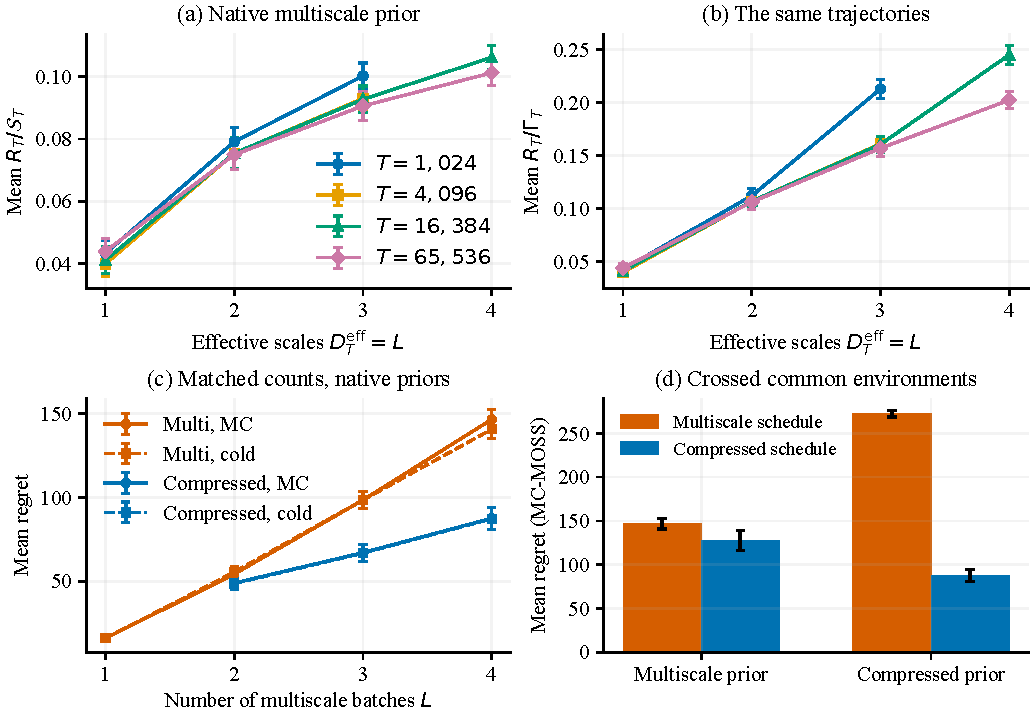
\includegraphics[width=\textwidth]{figures_v2/fig_geometry_risk.pdf}
 \caption{Bandit risk on a compatible finite product prior. Panels (a) and (b) use MC-MOSS and the native multiscale prior with gap multiplier four. Panel (c) compares each schedule under its native prior at $T=65536$; paired schedules have the same final count. Panel (d) fixes $T=65536$, $L=4$, and the sampled mean vector while changing its arrival schedule. Bars are $1.96$ Monte Carlo standard errors over 128 independent replications.}
 \label{fig:geometry-risk}
\end{figure}

\ifdefined\JASASubmission\FloatBarrier\fi
\subsection{Separating Clock Calibration, Capacity, and History}
\label{sec:mechanisms-experiments}

The next experiment separates the two changes hidden in a comparison with a
global-clock index.  We cross the clock, $s_t$ or $t$, with the capacity,
$d_j$ or $2(K_t-1)$, while retaining all observations in each of the four
rules.  Every rule uses the index
$\widehat\mu_i+\{\log_+(u_t/(v_tN_i))/N_i\}^{1/2}$, with the same
initialization and tie order.  MC-MOSS is the local-clock, frozen-capacity
cell.  A fifth rule uses precisely that cell but discards its observations
at the same capacity-doubling times.  These contrasts isolate finite-sample
effects; no spectral guarantee is asserted for the other three cells.

We also compare UCB1, AUER, Bernoulli KL-UCB, Thompson sampling, and clipped
MC-MOSS.  UCB1 and AUER use respective bonuses
$\{2\log(t)/N_i\}^{1/2}$ and $\{8\log(t)/N_i\}^{1/2}$
\citep{auer2002finite,kleinberg2008sleeping}.
KL-UCB uses the Bernoulli divergence and the original paper's recommended
experimental choice $c=0$ \citep{garivier2011kl}; Thompson sampling starts
each arriving arm with a $\operatorname{Beta}(1,1)$ prior
\citep{agrawal2012thompson}.  These are full-history arriving-arm
implementations of the stated rules.  We do not transfer their fixed-arm
guarantees to the present arrival model.

There are 32 candidates in batches of sizes $4,4,8,8,8$, arriving at
$1,\lfloor T/8\rfloor+1,\lfloor T/3\rfloor+1,
\lfloor T/2\rfloor+1,\lfloor3T/4\rfloor+1$, besides the initial anchor.
We fix five mean vectors: near ties, poor candidates, a persistent new
record at the fourth batch, a mixed-quality final batch, and an anchor at
the reward upper bound.  The full vectors are given in the supplement.
Both $T=2048$ and $T=8192$ are used.  Each cell has 128 independent
replications, coupled across methods by reward uniforms at each calendar
round.  We repeat the entire design with the order of labels reversed
within every candidate batch; the anchor remains first.  Parameters were
fixed before simulation, and software development used separate seeds.



Figure~\ref{fig:mechanisms-ablation} shows why the two factors must be
separated.  At $T=8192$, with forward labels and a mixed final batch, the
global clock costs $26.38$ (paired standard error $7.34$) relative to the
local clock when capacity is frozen.  With the global clock held fixed,
using current capacity reduces regret by $26.57$ ($1.30$).  The combined
global/current rule consequently has mean regret $224.24$, almost the
same as MC-MOSS's $224.42$, although the component contrasts are substantial.
Current capacity also improves on frozen capacity under the local clock,
by $18.90$ ($4.45$) in this example.  Thus the frozen capacity is a device
that supports the uniform analysis, not a claim of the best finite-sample
calibration.  Changing the clock to global increases mean regret in every
displayed cell, whereas discarding history is especially costly when
inferior candidates recur.  For poor candidates at $T=8192$, the latter
cost is $154.04$ ($2.12$).  Reversing labels preserves these broad patterns;
the near-tie differences at $T=2048$ are comparatively small and uncertain.

\begin{figure}[tbp]
\centering
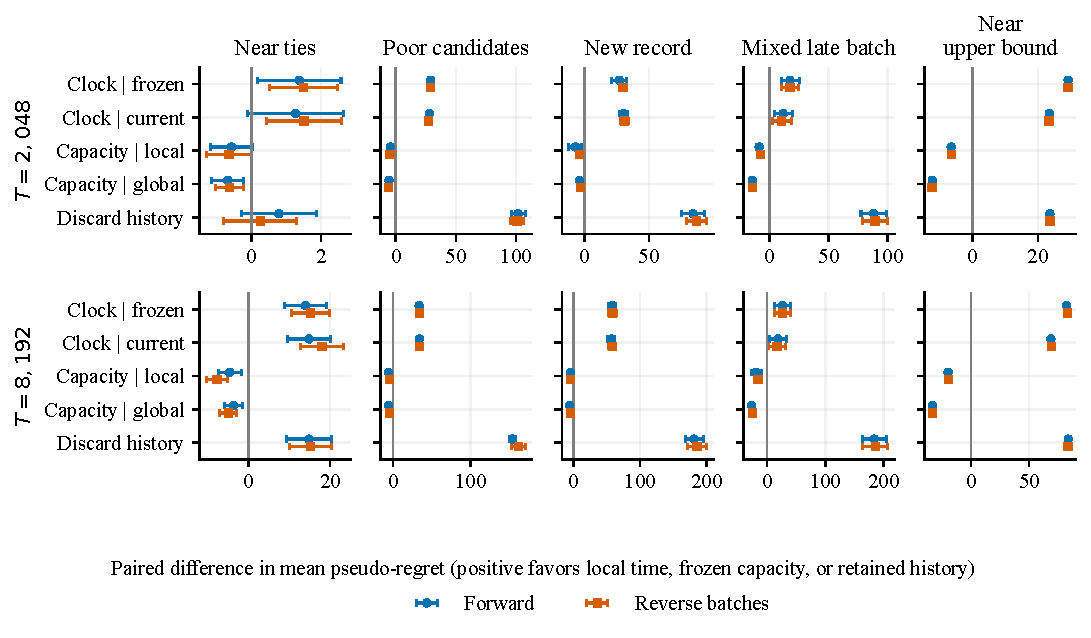
\includegraphics[width=\linewidth]{figures_v2/fig_mechanisms_ablation.pdf}
\caption{Matched mechanism contrasts under two horizons and two batch label
orders.  Clock contrasts are global minus local at fixed capacity;
capacity contrasts are current minus frozen at fixed clock.  Discarding
history is compared with MC-MOSS at identical reset times.  Points are
paired mean differences and bars are $1.96$ Monte Carlo standard errors
from 128 independent replications.  The intervals are pointwise, without
adjustment for the multiple displayed comparisons.  Horizontal scales
differ across panels.}
\label{fig:mechanisms-ablation}
\end{figure}

\begin{table}[t]
\centering
\caption{Pseudo-regret for four policies under five reward configurations.}
\label{tab:mechanisms-baselines}
\normalsize
\setlength{\tabcolsep}{3pt}
\begin{tabular*}{\linewidth}{@{\extracolsep{\fill}}lrrrr@{}}
\toprule
Configuration & MC-MOSS & KL-UCB & Thompson & Clipped MC \\
\midrule
Near ties & 103.85 (2.89) & 132.56 (0.50) & 125.81 (0.86) & 104.16 (2.69) \\
Poor candidates & 146.44 (0.86) & 236.00 (1.33) & 170.35 (1.12) & 147.36 (0.80) \\
New record & 157.11 (6.02) & 371.66 (3.06) & 242.72 (3.82) & 147.84 (4.55) \\
Mixed late batch & 224.42 (6.91) & 511.85 (5.57) & 304.10 (3.43) & 230.88 (7.33) \\
Near upper bound & 116.78 (0.36) & 1.70 (0.00) & 8.60 (0.30) & 0.00 (0.00) \\
\bottomrule
\end{tabular*}
\par\medskip\noindent\begin{minipage}{\linewidth}\normalsize\setstretch{1}
\textit{Notes:} Entries are mean pseudo-regret with Monte Carlo standard errors in parentheses at $T=8192$, forward labels, and 128 replications. The complete two-horizon, two-label-order results, including UCB1 and AUER, are in the computational supplement and released CSV files.
\end{minipage}
\end{table}


The stronger baselines also identify a substantial failure of the
unclipped rule (Table~\ref{tab:mechanisms-baselines}).  With anchor mean one
and candidate means $0.94$ or $0.985$, MC-MOSS incurs $116.78$ mean regret
at $T=8192$, compared with $1.70$ for KL-UCB and $8.60$ for Thompson sampling.
Clipped MC-MOSS has zero regret here: its indices never exceed one and
the specified tie rule keeps selecting the anchor.  This conclusion uses
the exact boundary mean and the anchor's priority; it is not an assertion
of uniform dominance by clipping.  Indeed, in the mixed-final-batch
configuration clipping changes regret by $6.46$ ($8.76$), with no resolved
improvement.  The comparisons support the roles of clock calibration and
history reuse while showing that a minimax guarantee leaves room for
large improvements on particular reward distributions.

\ifdefined\JASASubmission\FloatBarrier\fi
\subsection{A Common Environment Across Random Arrival Scales}\label{sec:experiment-random}
The third study holds the two reward means fixed before drawing the
arrival schedule. At $T=4^m$, $m=4,5,6,7$, the competing arm has lifetime
$H=4^J$, $J=0,\ldots,m$. We consider probabilities proportional to
$2^{-J}$, uniform scale probabilities, probabilities proportional to
$4^{-J}$, an equal mixture of the last two scales, and a point mass at
the last scale. The anchor mean is $1/2$; the competitor mean is
$1/2\pm\Delta$, with $\Delta=2^{-1-r/2}$, $r=0,\ldots,2m+2$.

One rule starts a fresh two-arm MOSS run with the remaining horizon
revealed by the known endpoint. The other is the original MC-MOSS,
which does not know the endpoint and retains all anchor observations.
Their panels specify this information difference. We simulate the
forced prefix exactly through its binomial sufficient statistic.

For each policy and mixture, we use 64 development replications to
select a single gap and sign, or a separate gap and sign for each lifetime.
Both selections are then evaluated on 128 independent replications per
lifetime. Mixture means use the known schedule probabilities, with
stratified Monte Carlo standard errors. A separate check draws 2048
actual schedules for each selected common environment. These are
held-out risks of development-selected members of a finite grid, not
estimates of the full minimax risk or of a continuous supremum.

Figure~\ref{fig:random-heatmap} shows the conditional risk of a better
arriving competitor. The difficult gap changes with the remaining
lifetime. The retained prefix changes this surface, so the two panels
also differ for reasons beyond endpoint information alone.
Figure~\ref{fig:random-common} then averages over the inverse-square-root
mixture. At the largest endpoint, fresh-horizon MOSS has held-out mean
regret 1.321 (standard error 0.018) under the selected common
environment, compared with 1.977 (0.026) when the selected
environment is allowed to depend on the schedule. The corresponding
geometric values are $W(Q)=1.412$ and $\mathbb E\sqrt H=4.016$.
The latter curve is an arrival-only reference, not an observed risk.

The remaining mixtures, direct schedule draws and selected gaps are
reported in the computational supplement. For the two-long-scale
mixture the held-out ordering is reversed: development selection can
miss the best grid member. Independent evaluation removes reuse of
selection noise from the reported means; it does not make finite-grid
selection exact. None of these finite experiments estimates an
asymptotic rate or establishes that the anytime policy attains the
random-template theorem.

\begin{figure}[tbp]
\centering
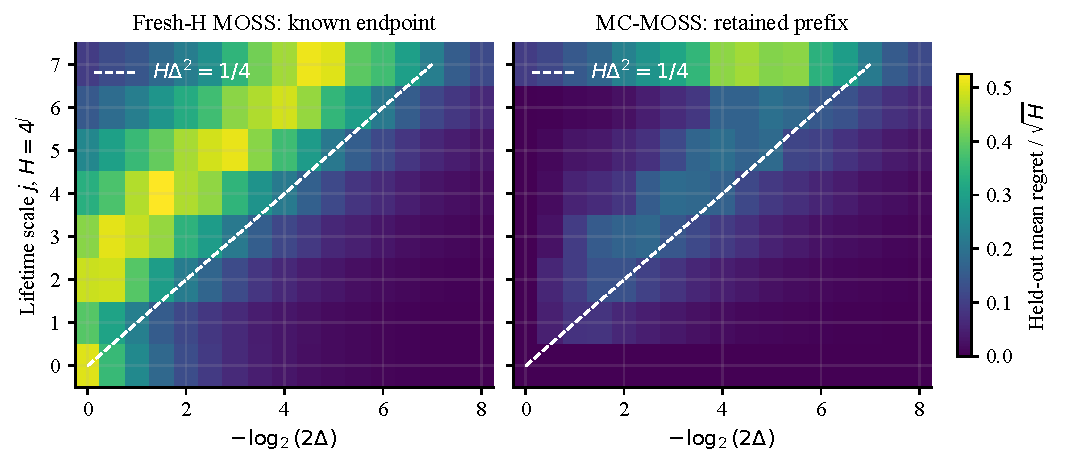
\includegraphics[width=\textwidth]{figures_v2/random_gap_heatmap.pdf}
\caption{Held-out regret divided by $\sqrt H$ for a better arriving
competitor at $T=16384$. Each cell uses 128 replications. The dashed
line marks $H\Delta^2=1/4$; it is a scale reference, not a fitted ridge.
The policies differ in endpoint knowledge and retention of the forced
anchor prefix.}\label{fig:random-heatmap}
\end{figure}
\begin{figure}[tbp]
\centering
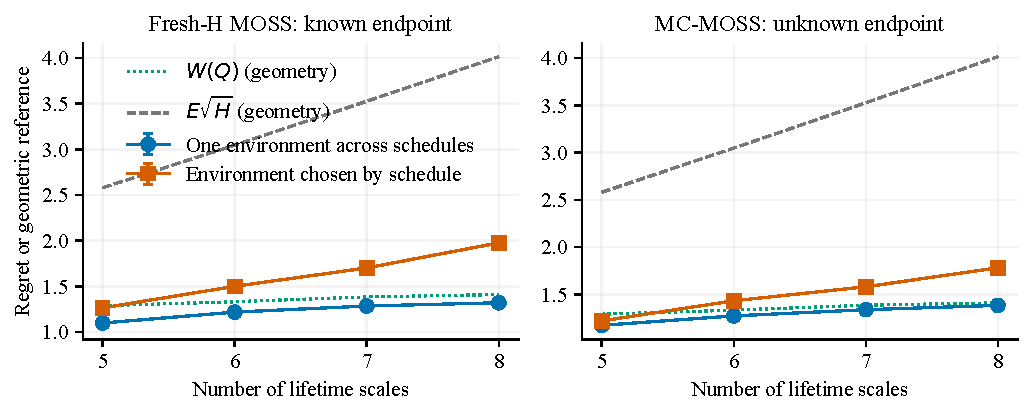
\includegraphics[width=\textwidth]{figures_v2/random_common_gap.pdf}
\caption{Common versus schedule-specific environments under
$\Pr(J=j)\propto2^{-j}$. Environments are selected on development
replications and evaluated independently. Bars are 1.96 stratified
Monte Carlo standard errors. The two geometric reference curves are
computed from the arrival law and are not risk estimates. Selection
is performed separately for each policy; the panels do not compare
the policies under one common mean vector.}
\label{fig:random-common}
\end{figure}

\ifdefined\JASASubmission\FloatBarrier\fi
\subsection{Two Fixed Batches Under a Random Common Stretch}
\label{sec:stretch-experiment}

We finally check the executable upper-bound construction on a template
with two batches of two candidates, $\boldsymbol\alpha=(4,1)$ and $K=5$.
Let $T=4\cdot4^m$, $m=3,4,5,6$, and let $H$ range over
$1,4,\ldots,4^m$.  We consider the inverse-square-root law
$\PP(H=4^j)\propto2^{-j}$, the uniform law on these scales, and the
deterministic longest scale.  Once the first batch arrives, the rule in
Theorem~\ref{thm:random-positive-main} runs fresh fixed-horizon MOSS experiments
of lengths $3H$ and $H$.  The comparison is the original anytime MC-MOSS,
which retains all observations, including the anchor's prefix.  The
former rule uses the known endpoint and revealed schedule; MC-MOSS is
given neither.

The fixed reward vector is
$(0.50,0.45,0.55,0.55+\eta\delta,0.50)$, with
$\eta\in\{-1,1\}$ and
$\delta\in\{0.025,0.05,0.10,0.20,0.40\}$.
For each $(m,Q)$ we use 64 development replications to select the single
pair $(\eta,\delta)$ with the largest law-averaged regret for the
revealed-stretch rule.  We evaluate that same pair on 128 independent
held-out replications for both policies and every value of $H$.
Thus no environment is selected after the realized stretch.  The finite
law is averaged exactly over its support, with Monte Carlo sampling only
for rewards.  These are held-out risks for selected common environments,
not estimates of the continuous minimax supremum.



At $m=6$, the inverse-square-root law has $W(Q)=1.386$;
the revealed-stretch rule has mean regret $5.94$ (standard error $0.05$),
and MC-MOSS has $3.11$ ($0.06$).  The corresponding revealed-stretch risks
are $39.81$ ($0.58$) under the uniform-scale law and $141.80$ ($3.14$)
under the deterministic longest scale, whose complexities are $12.190$
and $64$, respectively.  Figure~\ref{fig:stretch-heldout} displays the
normalized values across all four endpoints.  MC-MOSS performs better
in every selected cell, despite using less schedule information.  This
does not contradict the theorem: the reset construction proves an
upper bound and is not optimized for finite-sample constants.  Nor does
this finite grid establish the asymptotic rate or a matching lower
constant.  Its role is to verify that the common-environment averaging
and the multi-batch upper-bound rule can be implemented without
discarding regret incurred before the last batch.


\begin{figure}[tbp]
\centering
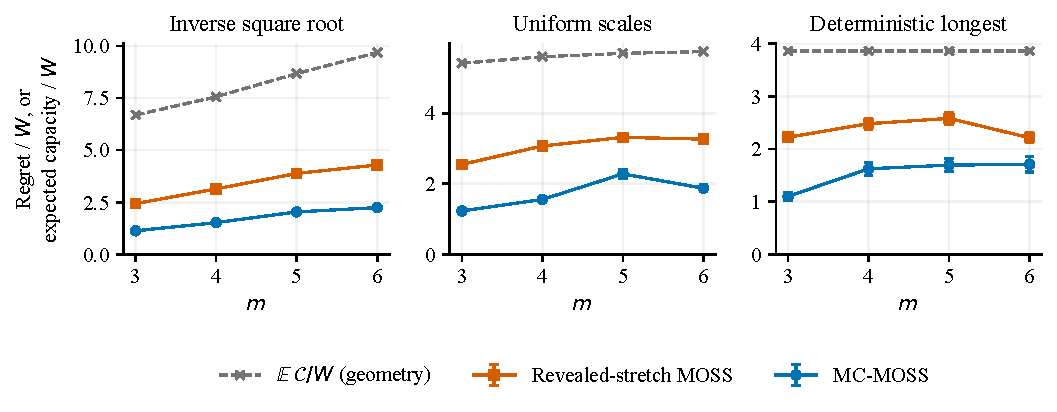
\includegraphics[width=\linewidth]{figures_v2/fig_stretch_heldout.pdf}
\caption{Held-out common-environment risks divided by $W(Q)$ for the
fixed two-batch template.  Error bars are $1.96$ Monte Carlo standard
errors under exact stratification over $H$.  The dashed curve is the
expected deterministic capacity divided by $W(Q)$ and is a geometric
reference, not an observed regret.  Both policies face the same
development-selected environment in each panel and at each $m$.}
\label{fig:stretch-heldout}
\end{figure}
\ifdefined\JASASubmission\FloatBarrier\fi

\section{Discussion}
The arrival schedule determines both which alternatives must be distinguished and how long their distinction can matter. For permanent arrivals with stationary bounded rewards, the schedule-specific minimax cost is an additive spectrum of remaining lifetimes. This result permits very late large batches to be inexpensive, while retaining the possibility that many separated scales each contribute to regret. An all-history causal policy achieves the resulting rate without estimating the future arrival process.

The allocation formulation gives a way to compare schedules before observing rewards. It can distinguish arrival plans with identical endpoints and arm counts, quantify the effect of timing perturbations, and express the marginal contribution of adding candidates. These are comparisons of worst-case learning difficulty. They do not measure the expected benefit of an arm whose mean is known or believed to be high. Using the capacity to design an admission policy would require a model for those benefits and a revised benchmark.

The mechanism experiments qualify how the optimal rate should guide implementation. Clock changes and capacity updates can have opposing finite-sample effects, so a comparison that changes both cannot identify either effect alone. Retaining observations avoids repeated exploration in some environments. The boundary examples and baseline comparisons show that the same minimax rate can conceal substantially different exploration costs near the reward upper bound. The gap bound depends on the smallest positive gaps and may be loose for heterogeneous instances. A general arrival-aware instance complexity, together with a policy attaining it, remains to be established.

The probability lower bound in the supplement shows that spectral difficulty is present with constant probability. The accompanying upper probability bounds come from expectation and are not sharp for small error probabilities. Likewise, the deterministic-time expectation bound alone makes no assertion at reward-dependent stopping times. Reward-dependent arrivals would also invalidate the simple conditioning and deterministic comparator-label arguments used here, and require a separate analysis.

Independent random arrivals change which hard environments can coexist. Theorem~\ref{thm:random-positive-main} resolves this issue for fixed, revealing batch templates: a truncated-lifetime functional replaces the average conditional capacity, and the ratio $D(Q)$ states when averaging is adequate. The result depends on a known endpoint and a fixed template, and its attaining policy uses the schedule information revealed by the first batch. A characterization for nonrevealing random schedules or for a growing collection of batches would have to account for information about future arrivals as well as information about reward means. The simulations illustrate the common-environment restriction without claiming to estimate that more general minimax problem.


\section*{Supplementary Material}
The mathematical supplement provides all proofs and additional probability and gap-dependent results. A separate computational supplement gives complete simulation designs, sensitivity analyses, baseline comparisons and the earlier fixed-endpoint study. The reproducibility package contains the policies, complexity calculations, simulation seeds, per-replicate results and scripts for every reported table and figure.

\section*{Data and Code Availability}
All numerical data in this article are generated by the accompanying Python scripts. The reconstruction package includes the complete source, environment versions, a master execution script and a mapping from scripts to reported outputs. It uses no restricted or external individual-level data.

\bibliographystyle{jasa-reference}
\bibliography{references}
\end{document}
